\documentclass{article}
\usepackage{amsmath}
\usepackage{amsthm}
\usepackage{amssymb}
\usepackage{enumerate}
\usepackage{graphicx}
% done
\begin{document}
    \title{MA3\_3 Exercise}
    \author{Wang Yue from CS Elite Class}
    \date{\today}

    \maketitle

    \section*{Exercise 3.10}

    \subsection*{6. Find the linear approximation of $f(x) = \sqrt[3]{1 + x}$ at $a = 0$ and use it to approximate the numbers $\sqrt{0.9}$ and $\sqrt{0.99}$. Illustrate by graphing $f$ and the tangent line.}

    $\because g'(x) = \frac 1 3 (1 + x)^{-\frac 2 3}, g(0) = \sqrt[3]{1} = 1, g'(0) = \frac 1 3$

    $\therefore$ the linear approximation of $g(x)$ at $a = 0$ is $$y - 1 = \frac 1 3(x - 0) \iff y = \frac 1 3 x + 1$$

    $\therefore \sqrt[3]{1 + x} \approx \frac 1 3 x + 1 \qquad $(when $x$ is near $0$)

    $\because 1 \approx 0.95$

    $\therefore $ let $x = -0.05$, and $$\sqrt[3]{1 - 0.05} = \sqrt[3]{0.95} \approx \frac{61}{60}$$

    $\because 1 \approx 1.1$
    
    $\therefore $ let $x = 0.1$, and $$\sqrt[3]{1 + 0.1} = \sqrt[3]{1.1} \approx \frac{31}{30}$$

    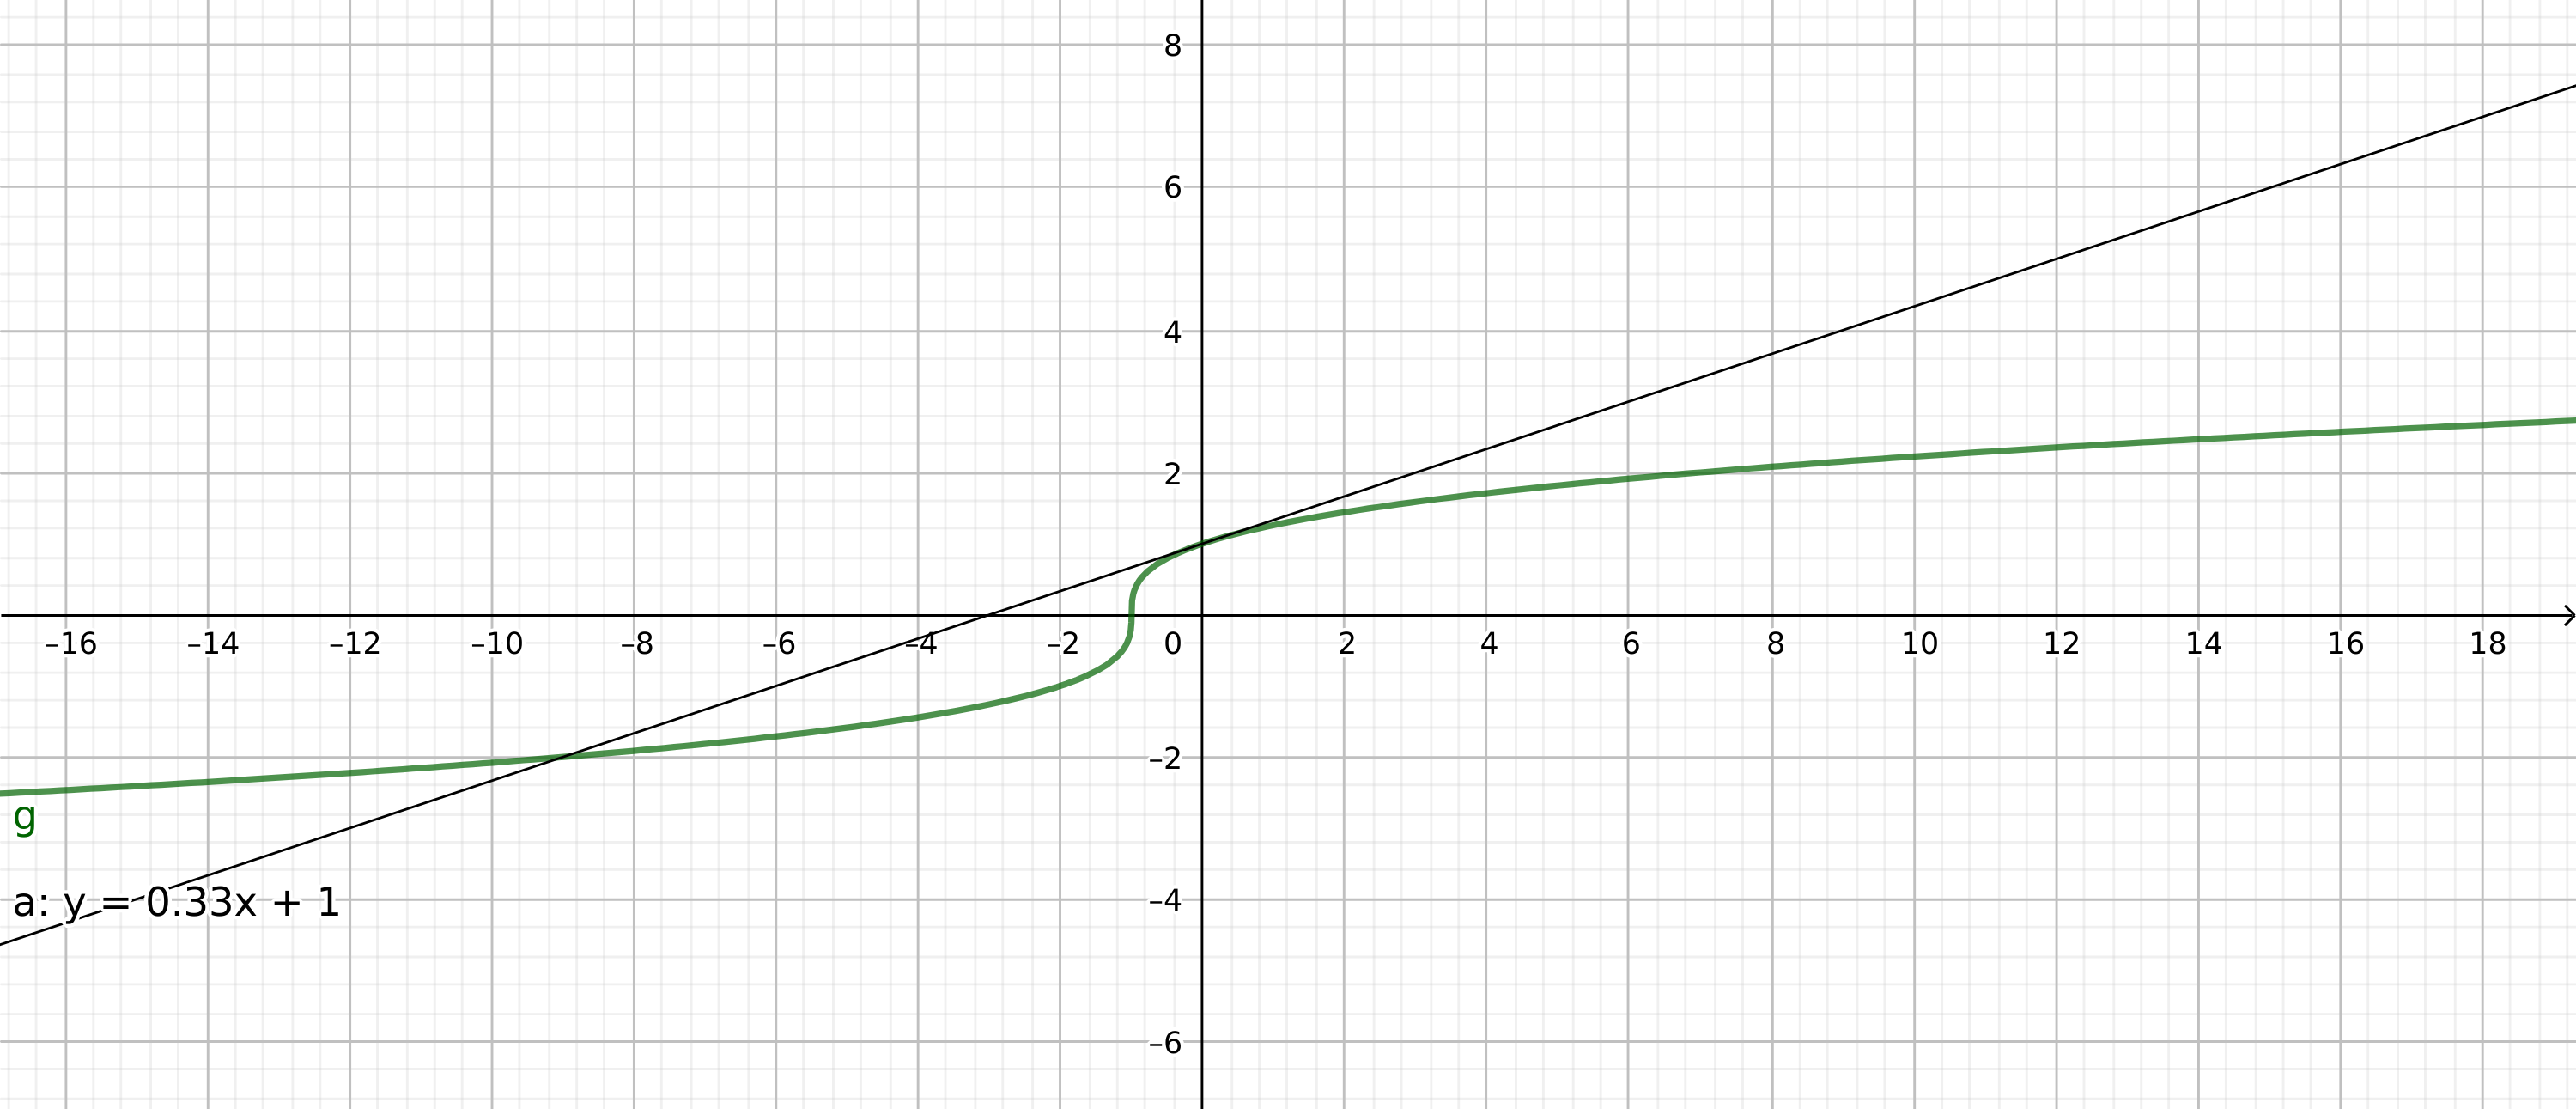
\includegraphics[scale=0.3]{6.png}

    \subsection*{11. (b) $y = \ln \sqrt{1 + x^2}$}

    $$\mathrm dy = \frac{1}{\sqrt{1 + x^2}} \frac{1}{2\sqrt{1 + x^2}} 2x \mathrm dx = \frac{x}{1 + x^2}\mathrm dx$$

    \subsection*{12. (a) $y = \frac{s}{1 + 2s}$}

    $$\mathrm dy = \frac{(1 + 2s) - 2s}{(1 + 2s)^2} \mathrm ds = \frac{1}{(1 + 2s)^2} \mathrm ds$$

    \subsection*{13. (a) $y = \tan \sqrt t$}

    $$\mathrm dy = \sec^2 (\sqrt t) \frac{1}{2\sqrt t} \mathrm dt = \frac{1}{2\sqrt t \cos^2 \sqrt t} \mathrm dt$$

    \subsection*{14. (a) $y = e^{\tan \pi t}$}

    $$\mathrm dy = e^{\tan \pi t} \sec ^2 (\pi t) \pi \mathrm dt = \frac{\pi e^{t \tan \pi t}}{\cos ^2 \pi t} \mathrm dt$$

    \subsection*{24. $e^{-0.015}$}

    $\because -0.015 \approx 0$

    $\therefore$ we can use the linear approximation of $e^x$ at $a = 0$

    $\because (e^x)'|_{x = 0} = 1, (e^x)|_{x = 0} = 1$
    
    $\therefore$ the linear approximation is $$y - 1 = 1(x - 0) \iff y = x + 1$$

    $\therefore e^x \approx x + 1 \qquad$(when $x$ is near $0$)

    $$\therefore e^{-0.015} \approx 1 - 0.015 = 0.985$$

    \subsection*{26. $\frac{1}{4.002}$}

    Let $f(x) = \frac{1}{x}$, and obviously $f'(x) = -\frac{1}{x^2}$

    $\because 4.002 \approx 4$

    $\therefore$ we can use linear approximation of $f(x)$ at $a = 4$

    $\because f'(4) = -\frac{1}{16}, f(4) = \frac 1 4$

    $\therefore$ the linear approximation is $$y - \frac 1 4 = -\frac{1}{16}(x - 4) \iff y = -\frac{1}{16}x + \frac{1}{2}$$

    $\therefore \frac 1 x \approx -\frac{1}{16}x + \frac 1 2 \qquad$(when $x$ is near $4$)

    $\therefore \frac{1}{4.002} \approx -\frac{4.002}{16} + \frac{1}{2} = \frac{6001}{8000}$

    % 6 11b 12a 13a 14a 24 26
\end{document}